\documentclass[a4paper, 11pt]{article}
\usepackage[polish]{babel}
\usepackage[MeX]{polski}
\usepackage[utf8]{inputenc}
\usepackage[T1]{fontenc}
%\usepackage{times}
\usepackage{graphicx,wrapfig}
\usepackage{pdfpages}
%\usepackage{anysize}
%\usepackage{tikz}
%\usetikzlibrary{calc,through,backgrounds,positioning}
\usepackage{anysize}
\usepackage{float}
%\usepackage{stmaryrd}
%\usepackage{amssymb}
%\usepackage{amsthm}
%\marginsize{3cm}{3cm}{3cm}{3cm}
%\usepackage{amsmath}
%\usepackage{color}
%\usepackage{listings}
%\usepackage{enumerate}


\begin{document}
	% \noindent -  w tym akapicie nie bedzie wciecia
	% \ indent - to jest aut., ale powoduje ze jest wciecie
	% \begin{flushleft}, flushright, center - wyrownianie akapitu
	% \textbf{pogrubiany tekst}
	% \textit{kursywa} 
	% 					STRONY 
	%  http://www.codecogs.com/latex/eqneditor.php 
	%  http://www.matematyka.pl/latex.htm
	% 
	\begin{titlepage}
	
	
		
		\newcommand{\HRule}{\rule{\linewidth}{0.5mm}} % Defines a new command for the horizontal lines, change thickness here
		
		\center % Center everything on the page
		
		%----------------------------------------------------------------------------------------
		%	HEADING SECTIONS
		%----------------------------------------------------------------------------------------
		
		\textsc{\LARGE Akademia Górniczo-Hutnicza im. Stanisława Staszica w Krakowie}\\[1.5cm] % Name of your university/college
		\textsc{\Large Inżynieria Oprogramowania}\\[1.5cm]
		%\textsc{\Large Krak�w}\\[0.5cm] % Major heading such as course name
		%\textsc{\large }\\[0.5cm] % Minor heading such as course title
		
		%----------------------------------------------------------------------------------------
		%	TITLE SECTION
		%----------------------------------------------------------------------------------------
		
		\HRule \\[0.4cm]
		{\fontsize{38}{50}\selectfont System Zarządzania Apteką}
	%	{ \Huge \bfseries} Symulator po�aru lasu\\[0.3cm] % Title of your document
		\HRule \\[5.5cm]
		
		%----------------------------------------------------------------------------------------
		%	AUTHOR SECTION
		%----------------------------------------------------------------------------------------
		
		% If you don't want a supervisor, uncomment the two lines below and remove the section above

\begin{minipage}{0.4\textwidth}
\begin{flushleft} \large 
\emph{Autorzy:}\\
Marcin \textsc{Jędrzejczyk}\\ % Your name
Paweł \textsc{Ogorzały} \\

\end{flushleft}
\end{minipage}
~
\begin{minipage}{0.4\textwidth}
\begin{flushright} \large
\emph{Prowadzący:}\\
 Dr inż. Radosław \textsc{Klimek}  % Supervisor's Name
\end{flushright}
\end{minipage} \\[5cm]

		
		%----------------------------------------------------------------------------------------
		%	DATE SECTION
		%----------------------------------------------------------------------------------------
		
		{\large \today}\\[3cm] % Date, change the \today to a set date if you want to be precise
		
		%----------------------------------------------------------------------------------------
		%	LOGO SECTION
		%----------------------------------------------------------------------------------------
		
		%\includegraphics{Logo}\\[1cm] % Include a department/university logo - this will require the graphicx package
		
		%----------------------------------------------------------------------------------------
		
		\vfill % Fill the rest of the page with whitespace
		
	\end{titlepage}
	
	%SPIS TRESI
	%
	%
	%
	%
	%
	%
	%
	%
	%
	
	\tableofcontents
	\vfill

	\newpage
	
	\section{Streszczenie systemu}
	\indent
	
	Nasz projekt przedstawia system zarządzania apteką. \newline
	\newline \indent 
	Apteka zapewnia obsługę klientów na miejscu.
	Klient ma możliwość zakupu leków bez recepty oraz z receptą. Płatności może dokonać za pomocą gotówki lub kartą. Klient może otrzymać fakturę bądź paragon.  \newline 
	\newline \indent
	Za obsługę klienta  odpowiada farmaceuta. W zakresie jego obowiązków leży także składanie zamówienia na lek w przypadku jeśli zauważy, że jego stan się kończy. Farmaceuta sporządza również raport z listą recept obsłużonych, którą wysyła do Narodowego Funduszu Zdrowia. \newline
	\newline \indent
	Za stan magazynu odpowiada magazynier. Tworzy on zamówienia i aktualizuje stan magazynu. \newline   
	\newline \indent
	Całość kontroluje kierownik, która ma możliwość zatrudniania oraz zwalniania pracowników. Kontroluje on także zamówienia składane przez magazyniera.	
	\section{Lista obiektów zewnętrznych}
	Obiekty zewnętrzne:
	\begin{itemize}
	\item Klient - posiada możliwość kupna leku za gotówkę lub kartą. Może on otrzymać paragon albo fakturę, a także zrezygnować z zakupu.
	\item Farmaceuta - jego zadaniem jest obsługa klienta. Ma obowiązek złożyć zamówienie na dostawę leku, jeżeli zauważy, że jest go mało na stanie lub kończy się jego termin ważności. Raz na miesiąc wysyła raport z listą numerów recept, które obsłużył do NFZ.
	\item Kierownik - ma możliwość zatrudniania pracowników. Kontroluje zamówienia składane przez magazyniera. Tylko on może dodać nowy lek do oferty apteki.
	\item Magazynier - jest osobą odpowiedzialną za bieżący stan magazynu. Ma możliwość sprawdzania magazynu, tworzenia zamówień, aktualizowania stanu magazynu.
	\item Narodowy Fundusz Zdrowia (NFZ)- do tej instytucji wysyłamy co miesiąc raport ze sprzedaży leków na receptę. 
	\end{itemize}
	\section{Lista zdarzeń}
	
	\begin{itemize}
	\item Wybór potwierdzenia wpłaty (paragon/faktura),
	\item Wybór formy płatności (gotówka/karta),
	\item Zrezygnowanie z kupna,
	\item Dokonanie płatności,
	\item Wybranie leku(recepta/bez recepty),
	\item Brak leku,
	\item Lek przeterminowany,
	\item Sporządzenie raportu,
	\item Przyjęcie dostawy leków.
	\end{itemize}
	
%	\section{Diagram kontekstowy}

	\section{Diagramy kontekstowy}
	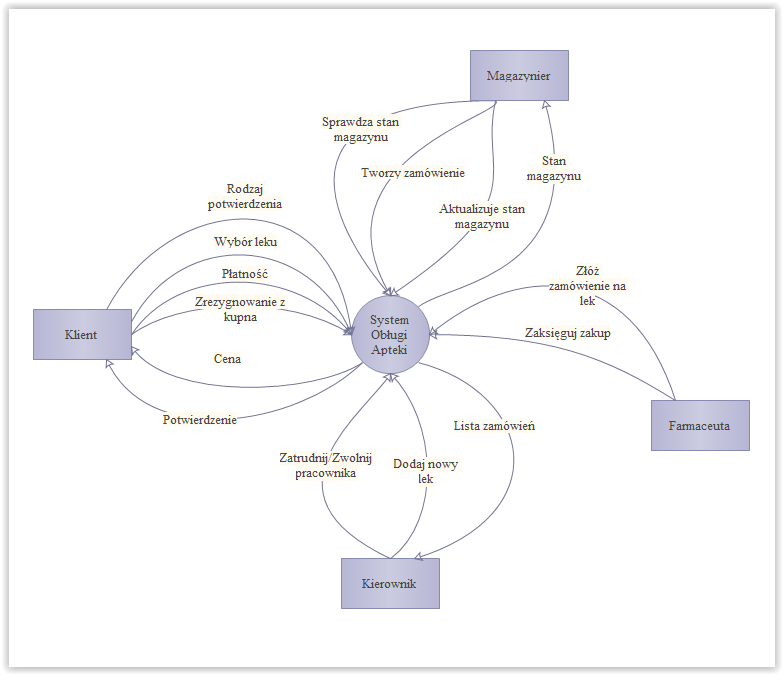
\includegraphics[scale=0.8]{zd.PNG} 
	\section{Diagram DFD-poziom 0}
		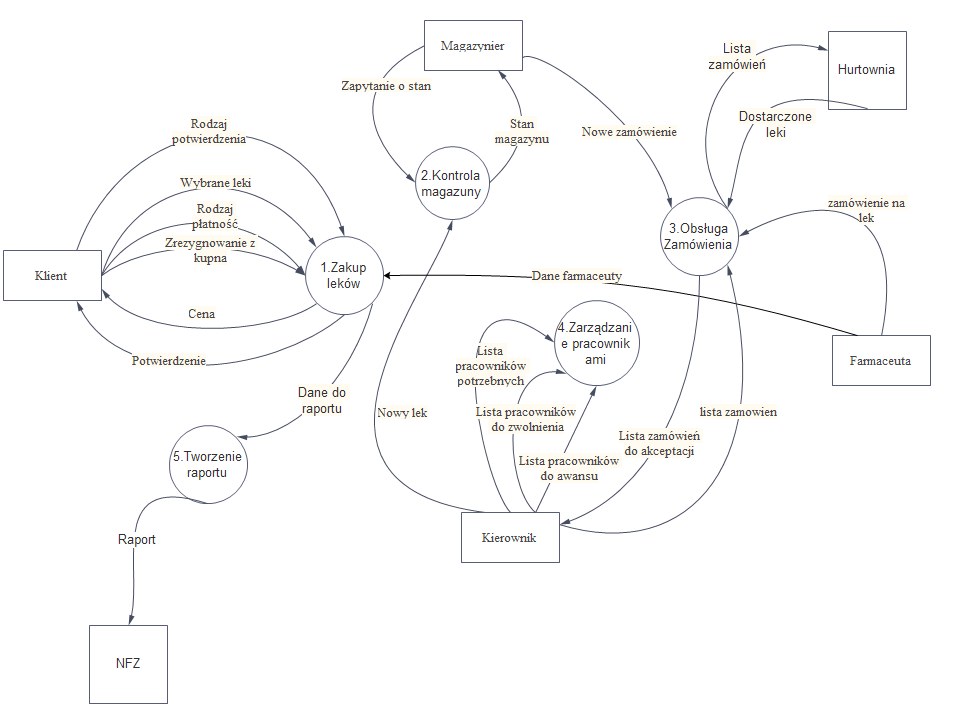
\includegraphics[scale=0.7]{dfdpoziom1.PNG} 
	
	\subsection{Diagram DFD - poziom 1 Kontrola magazynu}
		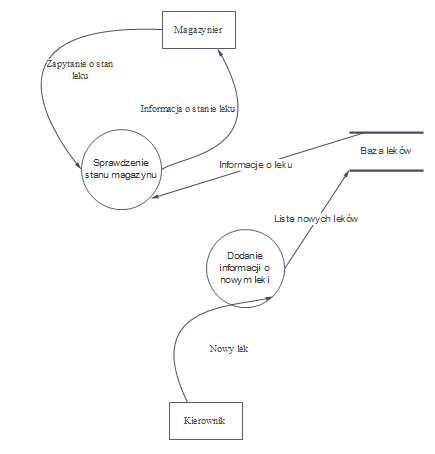
\includegraphics[scale=1]{kontrolaMagazynu.PNG} 
		
	\subsection{Diagram DFD - poziom 1 Zamówienia}
		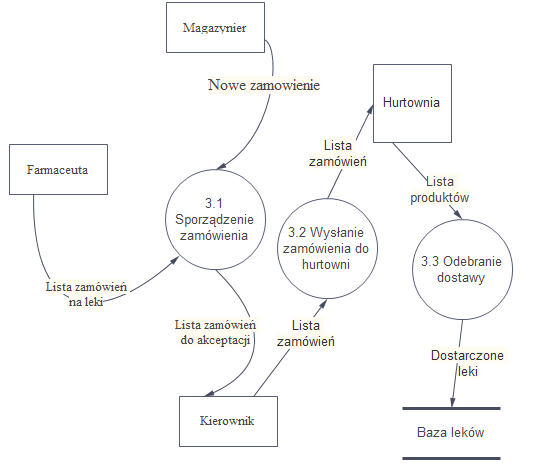
\includegraphics[scale=1]{zamowienia3.PNG} 
		
	\subsection{Diagram DFD - poziom 1 Zarządzanie pracownikami}
		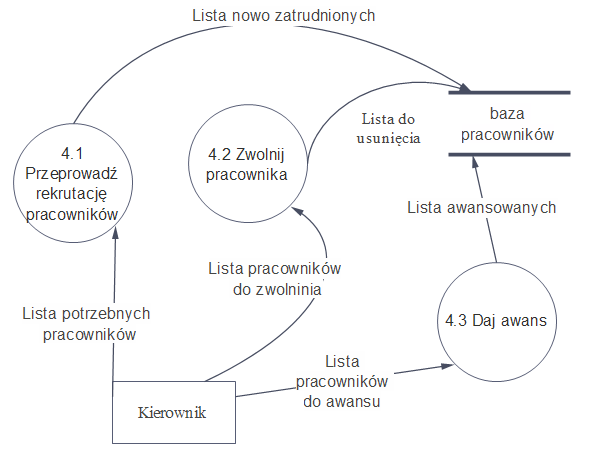
\includegraphics[scale=1]{zarzadzaniePracownikami2.PNG} 
		
	\subsection{Diagram DFD - poziom 1 Tworzenie raportu}
		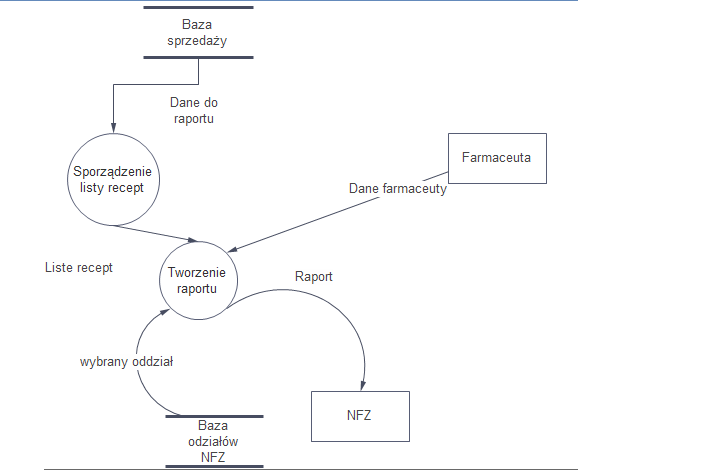
\includegraphics[scale=1]{tworzenieRaportu.PNG} 
		
	\subsection{Diagram DFD - poziom 1 Zakup leków}
		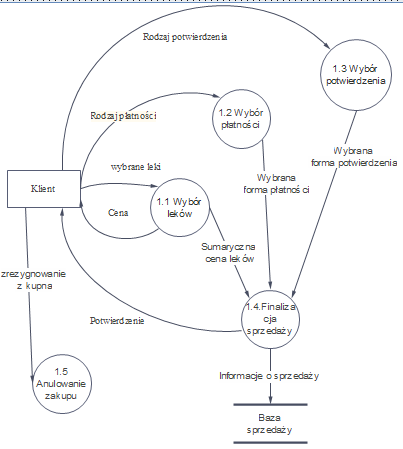
\includegraphics[scale=1]{zakupLekow2.PNG} 	
		\subsubsection{Poziom 2- Zakup leków- płatność gotówką}
			\begin{figure}[H]
			\centerline{\includegraphics[scale=1]{dfdp21.png}}
			\caption{Diagram STD dla raportu}
			\end{figure}
		\subsubsection{Poziom 2- Zakup leków- płatność kartą}
			\begin{figure}[H]
			\centerline{\includegraphics[scale=1]{dfdp22.png}}
			\caption{Diagram STD dla raportu}
			\end{figure}
			
	\section{Model danych diagram ERD}
	
			\begin{figure}[H]
			\centerline{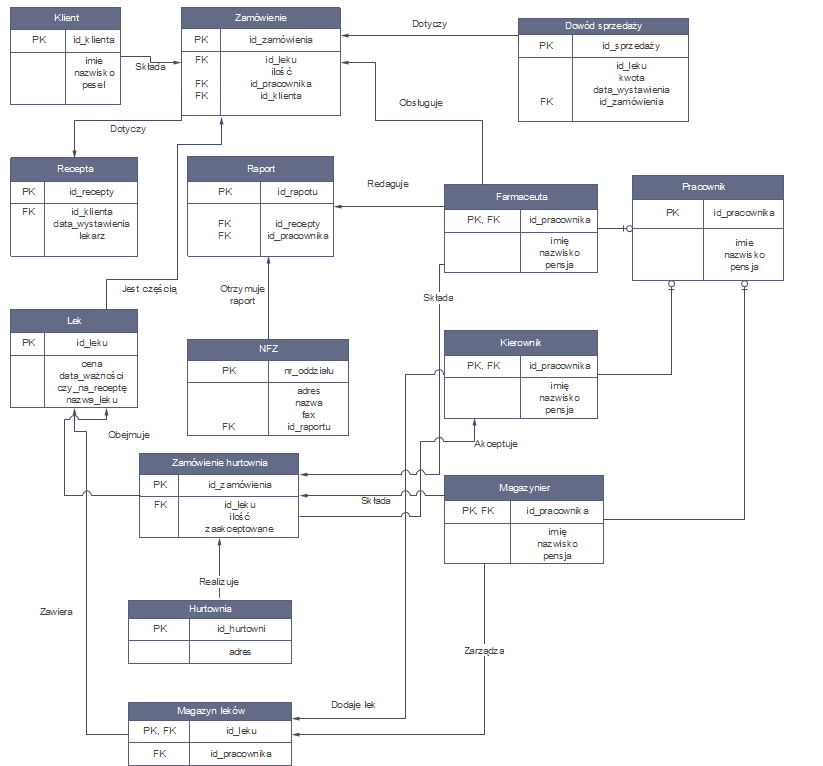
\includegraphics[scale=1]{ERD.png}}
			\caption{Diagram ERD apteki}
			\end{figure}
	\subsection{Opis atrybutów encji}
	%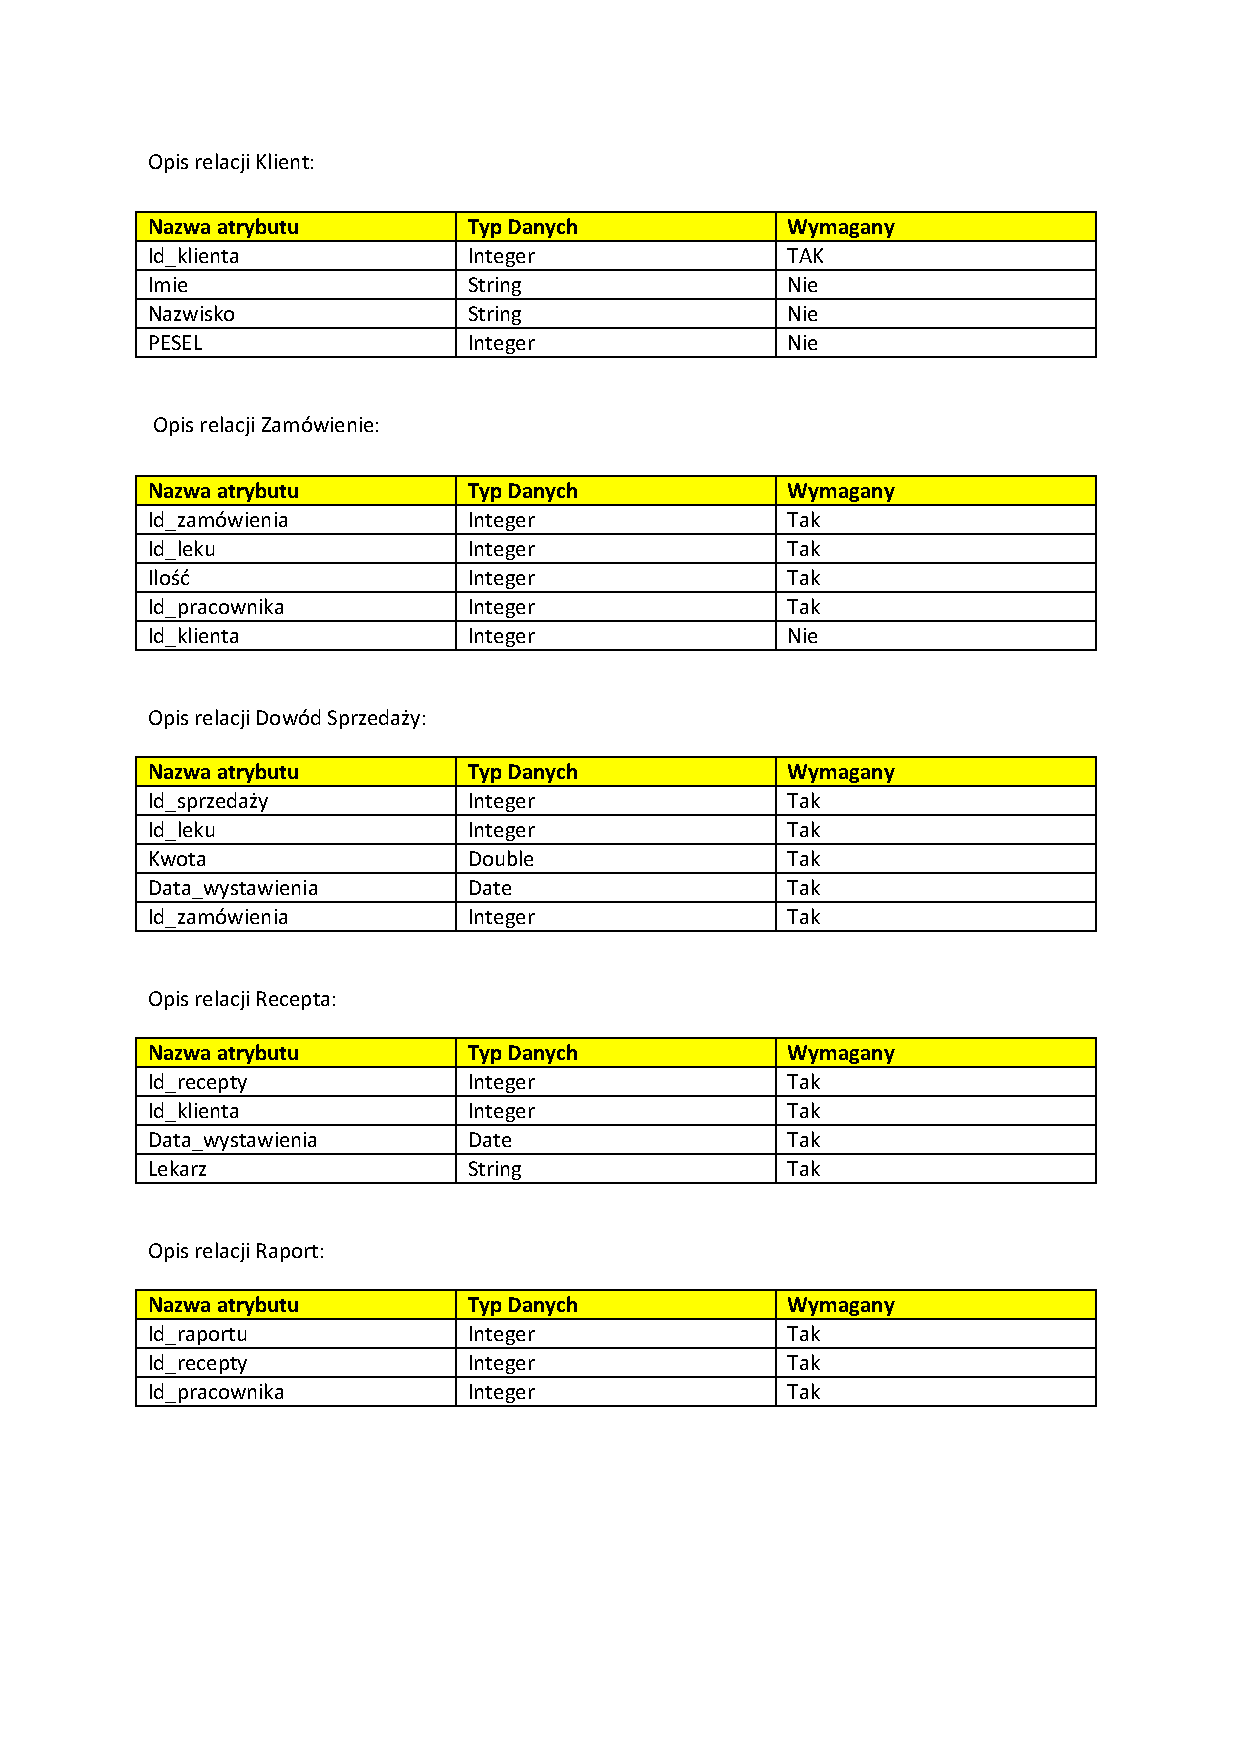
\includepdf[pages=-]{opisERD.pdf}
 Klient\\
\begin{tabular}{|l|l|l|} \hline
Nazwa  atrybutu	& Typ Danych	& Wymagany \\ \hline
Id\_klienta	& Integer	& Tak \\ \hline
Imie & 	String	& Nie \\ \hline
Nazwisko & String &	Nie \\ \hline
PESEL 	& 	Integer	& Nie \\ \hline
\end{tabular}\\[1cm]

Zamówienie\\
\begin{tabular}{|l|l|l|} \hline
Nazwa  atrybutu	& Typ Danych	& Wymagany \\ \hline
Id\_zamówienia	 &Integer	& Tak \\ \hline
Id\_leku &	Integer	& Tak\\ \hline
Ilość	& Integer	& Tak\\ \hline
Id\_pracownika &	Integer	& Tak\\ \hline
Id\_klienta &	Integer &	Tak\\ \hline
\end{tabular}\\[1cm]
	
Dowód sprzedaży\\
\begin{tabular}{|l|l|l|} \hline
Nazwa   atrybutu	& Typ Danych	& Wymagany \\ \hline
Id\_sprzedaży	& Integer &	Tak\\ \hline
Id\_leku &	Integer	& Tak\\ \hline
Kwota	& Double &	Tak\\ \hline
Data\_wystawienia	& Date	& Tak\\ \hline
Id\_zamówienia	& Integer	& Tak\\ \hline
\end{tabular}\\[1cm]

Recepta\\
\begin{tabular}{|l|l|l|} \hline
Nazwa   atrybutu	& Typ Danych	& Wymagany \\ \hline
Id\_recepty &	Integer	& Tak\\ \hline
Id\_klienta	& Integer	 &Tak\\ \hline
Data\_wystawienia& 	Date	 &Tak\\ \hline
Lekarz &	String &	Tak\\ \hline
\end{tabular}\\[1cm]	
\newpage
Raport\\
\begin{tabular}{|l|l|l|} \hline
Nazwa   atrybutu	& Typ Danych	& Wymagany \\ \hline
Id\_raportu	& Integer	& Tak\\ \hline
Id\_recepty	& Integer	& Tak\\ \hline
Id\_pracownika	& Integer	& Tak\\ \hline
\end{tabular}\\[1cm]	

Pracownik \\
\begin{tabular}{|l|l|l|} \hline
Nazwa   atrybutu	& Typ Danych	& Wymagany \\ \hline
Id\_pracownika	& Integer	& TAk\\ \hline
Imię	& String	& Tak\\ \hline
Nazwisko	& String	& Tak\\ \hline
Pensja	& Integer	& Nie\\ \hline
\end{tabular}\\[1cm]	

Kierownik (dziedziczy po Pracownik)\\
\begin{tabular}{|l|l|l|} \hline
Nazwa  atrybutu	& Typ Danych	& Wymagany \\ \hline
Id\_pracownika	& Integer	& TAk\\ \hline
Imię	& String	& Tak\\ \hline
Nazwisko	& String	& Tak\\ \hline
Pensja	& Integer	& Nie\\ \hline
\end{tabular}\\[1cm]	

Magazynier (dziedziczy po Pracownik)\\
\begin{tabular}{|l|l|l|} \hline
Nazwa  atrybutu	& Typ Danych	& Wymagany \\ \hline
Id\_pracownika	& Integer	& TAk\\ \hline
Imię	& String	& Tak\\ \hline
Nazwisko	& String	& Tak\\ \hline
Pensja	& Integer	& Nie\\ \hline
\end{tabular}\\[1cm]	

Farmaceuta (dziedziczy po Pracownik)\\
\begin{tabular}{|l|l|l|} \hline
Nazwa  atrybutu	& Typ Danych	& Wymagany \\ \hline
Id\_pracownika	& Integer	& TAk\\ \hline
Imię	& String	& Tak\\ \hline
Nazwisko	& String	& Tak\\ \hline
Pensja	& String	& Nie\\ \hline
\end{tabular}\\[1cm]

Lek\\
\begin{tabular}{|l|l|l|} \hline
Nazwa  atrybutu	& Typ Danych	& Wymagany \\ \hline
Id\_leku	& Integer	&Tak\\ \hline
Cena	&Double	&Nie\\ \hline
Data\_ważności	&Date	&Tak\\ \hline
Czy\_na\_recepte &	Boolean	&Tak\\ \hline
Nazwa\_leku	&String	&Tak\\ \hline
\end{tabular}\\[1cm]	

NFZ\\
\begin{tabular}{|l|l|l|} \hline
Nazwa  atrybutu	& Typ Danych	& Wymagany \\ \hline
Nr\_odzdziału	&Integer	&Tak\\ \hline
Adres	&String&	Tak\\ \hline
Nazwa	&String&	Tak\\ \hline
Fax	&Integer&	Nie\\ \hline
Id\_raportu	&Integer	&Tak\\ \hline
\end{tabular}\\[1cm]	

Zamówienie hurtownia\\
\begin{tabular}{|l|l|l|} \hline
Nazwa  atrybutu	& Typ Danych	& Wymagany \\ \hline
Id\_zamówienia	&Integer	&Tak\\ \hline
Id\_leku	&Integer	&Tak\\ \hline
Ilość	&Integer	&Tak\\ \hline
Zaakceptowane	&Boolean	&Tak\\ \hline
\end{tabular}\\[1cm]	

Hurtownia\\
\begin{tabular}{|l|l|l|} \hline
Nazwa   atrybutu	& Typ Danych	& Wymagany \\ \hline
Id\_hurtowni &	Integer	&Tak\\ \hline
Adres&	String&	Tak\\ \hline
\end{tabular}\\[1cm]	

Magazyn leków\\
\begin{tabular}{|l|l|l|} \hline
Nazwa  atrybutu	& Typ Danych	& Wymagany \\ \hline
Id\_leku	&Integer	&Tak\\ \hline
Id\_pracownika	&Integer	&Tak\\ \hline
\end{tabular}\\[1cm]	


	\section{Model dynamiki systemu Diagramy STD}
	\begin{figure}[H]
\centerline{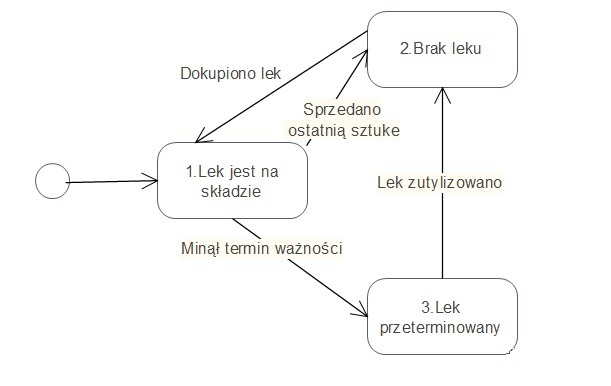
\includegraphics[scale=1]{STDlek.jpg}}
\caption{Diagram STD dla leku}
\end{figure}
	\begin{figure}[H]
\centerline{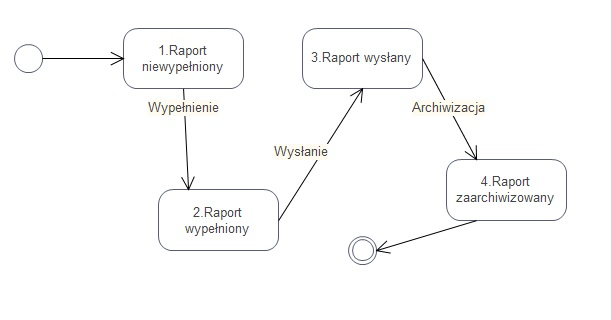
\includegraphics[scale=1]{STDraport.jpg}}
\caption{Diagram STD dla raportu}
\end{figure}

	\begin{figure}[H]
\centerline{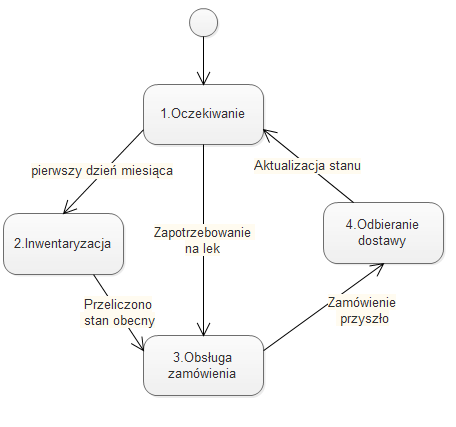
\includegraphics[scale=1]{STDmagazyn.png}}
\caption{Diagram STD dla magazynu}
\end{figure}
	\begin{figure}[H]
\centerline{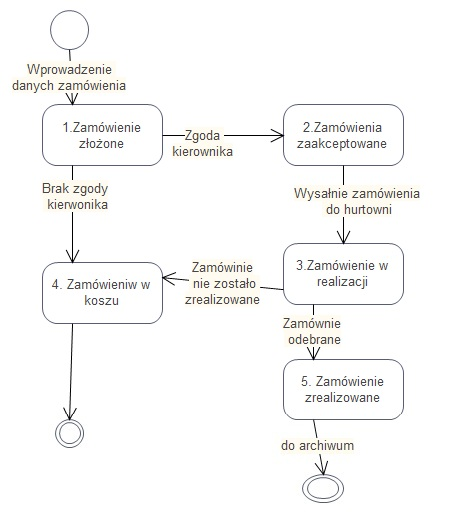
\includegraphics[scale=1]{STDzamowienie2.jpg}}
\caption{Diagram STD dla obsługi zamówienia z magazynu}
\end{figure}

	\begin{figure}[H]
\centerline{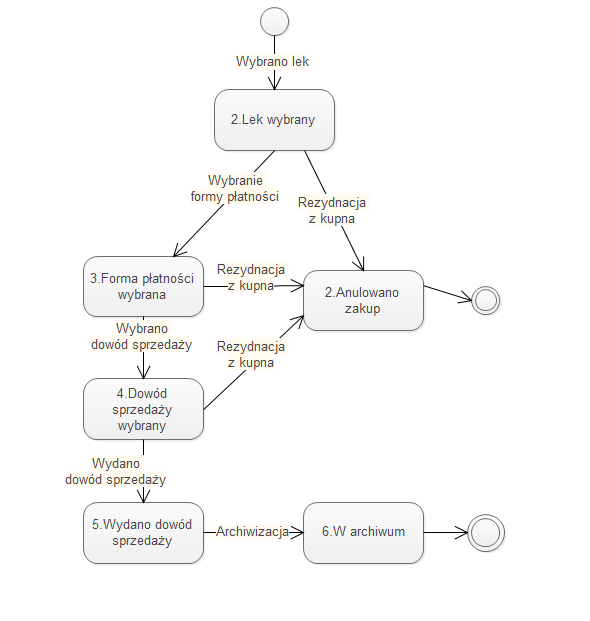
\includegraphics[scale=1]{STDzakup.png}}
\caption{Diagram STD dla zakupu leku}
\end{figure}
	\section{Słowniki danych}
	\textbf{C} \newline \newline
	\noindent
	cena = {cyfra} + waluta \newline
	cyfra = ["0" | "1" \textpipe "2" \textpipe "3" \textpipe "4" \textpipe "5" \textpipe "6" \textpipe "7" \textpipe "8" \textpipe "9"] \newline \newline
	\textbf{D} \newline \newline
	\noindent
	dane do raportu = {dowód sprzedaży} \newline
	dane farmaceuty = \at id\_pracownika + imię + nazwisko \newline
	dane karty = {cyfra} \newline
	dane przelewu = {cyfra} \newline
	dostarczone leki = "patrz:nowe zamówienie" \newline
	dowód sprzedaży = \at id\_sprzedaży + id\_leku + kwota + data\_wystawienia + id\_zamówienia \newline \newline
	\textbf{I} \newline \newline
	\noindent
	informacja o stanie leku = "patrz:lek" \newline
	informacje o leku = "patrz:lek" \newline
	informacje o sprzedaży = "patrz:dowód sprzedaży" \newline \newline
	\textbf{K} \newline \newline
	\noindent
	kwota reszty = "patrz:cena" \newline
	kwota zapłaty = "patrz:cena" \newline \newline
	\textbf{L} \newline \newline
	\noindent
	lek = \at id\_leku + cena + data\_ważności + czy\_na\_receptę + nazwa\_leku \newline
	lista awansowanych = "patrz:lista pracowników" \newline
	lista do usunięcia = "patrz:lista pracowników" \newline
	lista nowo zatrudnionych = "patrz:lista pracowników" \newline
	lista nowych leków = nowy lek + ilość \newline
	lista potrzebnych pracowników = stanowisko + ilość \newline
	lista pracowników = {pracownik} \newline
	lista pracowników do awansu = "patrz:lista pracowników" \newline
	lista pracowników do zwolnienia = "patrz:lista pracowników" \newline
	lista produktów = "patrz:nowe zamówienie" \newline
	lista recept = {recepta} \newline
	lista zamówień = "patrz:nowe zamówienie" \newline
	lista zamówień do akceptacji = "patrz:nowe zamówienie" \newline
	lista zamówień na leki = "patrz:nowe zamówienie" \newline \newline
	\textbf{N} \newline\newline
	\noindent
	nowe zamówienie = lek + ilość \newline
	nowy lek = "patrz:lek" \newline
	numer wpłaty = {cyfra} \newline \newline
	\textbf{P} \newline \newline
	\noindent
	potwierdzenie = "patrz:rodzaj potwierdzenia" \newline
	potwierdzenie dokonania płatności = "patrz:dowód płatności" \newline
	potwierdzenie dokonania przelewu = "Potwierdzono" \newline
	pracownik = \at id\_pracownika + imię + nazwisko + (pensja) \newline \newline
	\textbf{R} \newline \newline
	\noindent	
	raport = \at id\_raportu + id\_recepty + id\_pracownika \newline
	recepta = \at id\_recepty + id\_klienta + data\_wystawienia + lekarz \newline
	rodzaj płatności = ["Gotówka" \textpipe "Karta"] \newline
	rodzaj potwierdzenia = ["Rachunek" \textpipe "Faktura"] \newline \newline
	\textbf{S} \newline \newline
	\noindent
	stanowisko = ["Magazynier" \textpipe "Farmaceuta" \textpipe "Kierownik"] \newline
	sumaryczna cena leków = "patrz:cena" \newline \newline
	\textbf{W} \newline \newline
	\noindent
	waluta = ["Euro \textpipe "PLN"] \newline
	wybrana forma płatności = "patrz:rodzaj płatności" \newline
	wybrana forma potwierdzenia = "patrz:rodzaj potwierdzenia" \newline
	wybrane leki = {lek} \newline
	wybrany oddział = \at nr\_oddziału \newline \newline
	\textbf{Z} \newline \newline
	\noindent	
	zapytanie o stan leku = "patrz:lek" \newline
	zrezygnowanie z kupna = ["Tak" \textpipe "Nie"] \newline \newline
	
	\section{Specyfikacja procesów PSPEC}


	\begin{enumerate}	
	\item  Zakup leków
	\begin{enumerate}
	\item 1.1 Wybór leków\\
	Dane wejściowe: wybrane leki.\\	
	Warunek wejściowy: lek jest na składzie.\\	
	Opis działania:\\
		Podliczamy sumę wybranych przez klienta leków i pokazujemy mu ją jako cenę. Wysyłamy sumaryczną cenę leków do procesu finalizacji.\\
		
	Dane wyjściowe: cena, sumaryczna cena leków.\\	
	Warunek wyjścia:brak.\\	
	
	\item 1.2 Wybór płatności\\
	Dane wejściowe: rodzaj płatności.\\
	Warunek wejściowy: brak.\\
	Opis działania:\\
		Przygotowujemy się na sposób w jaki zapłaci nam klient.\\
		
	Dane wyjściowe: wybrana forma płatności.\\
	Warunek wyjścia: brak.\\	
	\item 1.3 Wybór potwierdzenia\\
	Dane wejściowe: rodzaj potwierdzenia.\\
	Warunek wejściowy: brak.\\
	Opis działania:\\
		Przygotowujemy odpowiedni formularz dowodu sprzedaży zgodny z wybranym przez klienta rodzajem potwierdzenia.\\
		
	Dane wyjściowe:wybrana forma potwierdzenia \\
	Warunek wyjścia: brak\\	
	\item 1.4 Finalizacja sprzedaży
	\begin{enumerate}
	\item  1.4.1 Płatność gotówką
		\begin{enumerate}
			\item 1.4.1.1 Wpłacenie pieniędzy do kasy\\

	Dane wejściowe: sumaryczna cena leków,wybrana forma płatności,wybrana forma potwierdzenia .\\
	Warunek wejściowy: wybrana forma płatności to gotówka, sumaryczna cena leków jest niższa bądź równa kwocie zapłaty .\\
	Opis działania:\\
		Klient wpłaca kwotę zapłaty w gotówce do kasy fiskalnej. Kasa oblicza nam resztę do wydania, która jest przekazywana klientowi wraz z dowodem sprzedaży w formie przez niego wybranej(wybrana forma potwierdzenia). Informacje o sprzedaży zapisujemy w historii w bazie sprzedaży.\\
		
	Dane wyjściowe: dowód sprzedaży, kwota reszty, kwota zapłaty,informacje o sprzedaży. \\
	Warunek wyjścia: brak.\\	
		\item 1.4.2 Płatność kartą
		\begin{enumerate}
		\item 1.4.2.1 Wykonanie zapłaty kartą\\
	Dane wejściowe: sumaryczna cena leków,wybrana forma płatności,wybrana forma potwierdzenia .\\
	Warunek wejściowy: wybrana forma płatności to karta płatnicza.\\
	Opis działania:\\
		Klient korzysta z terminala kart, aby zapłacić za wybrane przez siebie leki. Przygotowywany jest dowód sprzedaży.\\
		
	Dane wyjściowe: Dane karty,przelewu,numer wpłaty \\
	Warunek wyjścia: brak.\\	
	
		\item 1.4.2.2 Potwierdzenie zapłaty\\
	Dane wejściowe: numer wpłaty, potwierdzenie dokonania przelewu .\\
	Warunek wejściowy: brak.\\
	Opis działania:\\
		Sprawdzamy, czy dokonano przelewu. Jeśli tak, to drukujemy potwierdzenie i przekazujemy je wraz z dowodem sprzedaży klientowi, kopie zachowując dla siebie \\
		
	Dane wyjściowe: potwierdzenie dokonania płatności. \\
	Warunek wyjścia: brak.\\	
		\end{enumerate}
		\end{enumerate}
	\end{enumerate}
	
	
		
		
	\item 1.5 Anulowanie zakupu\\
	Dane wejściowe: zrezygnowanie z kupna.\\
	Warunek wejściowy: brak.\\
	Opis działania:\\
		Wycofanie informacji przekazanych przez klienta do tej pory z transakcji i anulowanie jej. \\
	Dane wyjściowe: brak.\\
	Warunek wyjścia: brak.\\	
	\end{enumerate}
	
	\item Kontrola magazynu
	\begin{enumerate}
	\item 2.1 Sprawdzenie stanu magazynu\\
	Dane wejściowe: Zapytanie o stan leku, informacje o leku.\\
	Warunek wejściowy: brak.\\
	Opis działania:\\
		Algorytm obsługuje zapytanie o stan leku i sprawdza informacje o nim w bazie leków, po czym wysyła informację zwrotną o stanie leku\\
	Dane wyjściowe: informacje o stanie leku.\\
	
	Warunek wyjścia: brak.\\
	\item 2.2 Dodanie informacji o nowym leku\\
	Dane wejściowe: nowy lek.\\
	Warunek wejściowy: brak.\\
	Opis działania:\\
		Algorytm dostaje informacje o nowym leku. Sprawdza ich poprawność. Po czym tworzy dla niego rekord zgodny z tabelą lek i wysyła go do bazy leków. \\
		
	Dane wyjściowe: lista nowy leków.\\
	Warunek wyjścia: brak.\\
\end{enumerate}		
	
	
	\item Zamówienia
	\begin{enumerate}
		\item 3.1 Sporządzenie zamówienia\\
	Dane wejściowe: nowe zamówienie, lista zamówień na leki.\\
	Warunek wejściowy: brak.\\
	Opis działania:\\
		Wypełnienie formularza zamówienia na nowe leki danymi przekazanymi przez farmaceutę oraz magazyniera. Następnie wysłanie formularza do kierownika.\\
		
	Dane wyjściowe: Lista zamówień do akceptacji.\\
	Warunek wyjścia: lista nie jest pusta.\\
		\item 3.3 Wysłanie zamówienia do hurtowni	
	Dane wejściowe: lista zamówień.\\
	Warunek wejściowy: lista jest zaakceptowana.\\
	Opis działania:\\
		Lista zamówień zaakceptowanych przez kierownika zostaje wysłana do hurtowni.\\
		
	Dane wyjściowe: lista zamówień. \\
	Warunek wyjścia: brak\\
		\item 3.4 Odebranie dostawy
	Dane wejściowe: lista produktów.\\
	Warunek wejściowy: brak.\\
	Opis działania:\\
		Wykonanie formalności związanych z odbieraniem dostawy od hurtownika. Sprawdzenie dostarczonych produktów i zapłacenie za nie. Dodanie informacji o dostarczonych lekach do bazy leków. \\
		
	Dane wyjściowe: Dostarczone leki\\
	Warunek wyjścia: brak.\\
	\end{enumerate}
	
	
	\item Zarządzanie pracownikami\\
	\begin{enumerate}
	\item 4.1 Przeprowadź rekrutację pracowników	\\
	Dane wejściowe: Lista potrzebnych pracowników.\\
	Warunek wejściowy: lista nie jest pusta.\\
	Opis działania:\\
		Dostajemy informację jakich pracowników poszukujemy. Sprawdzamy nadesłane do nas CV. Zapraszamy na rozmowę kwalifikacyjną osoby, które nadają się na stanowiska z wakatem. Zatrudniamy odpowiednie osoby. Tworzymy listę nowo zatrudnionych osób, po czym wysyłamy ją do bazy pracowników. \\
		
	Dane wyjściowe: lista nowo zatrudnionych.\\
	Warunek wyjścia: Zatrudniono pracownika.\\
	
		\item 4.2 Zwolnij pracownika\\
	Dane wejściowe: Lista pracowników do zwolnienia.\\
	Warunek wejściowy: lista nie jest pusta.\\
	Opis działania:\\
		Rozwiązujemy umowę z pracownikami z listy i dopełniamy formalności prawnych z tym związanych. Po czym aktualizujemy bazę pracowników aktualnie zatrudnionych. \\
		
	Dane wyjściowe: lista do usunięcia.\\
	Warunek wyjścia: Zwolniono pracownika.\\
		
		\item 4.3 Daj awans	\\
	Dane wejściowe: Lista pracowników do awansu.\\
	Warunek wejściowy: lista nie jest pusta.\\
	Opis działania:\\
		Dajemy awans pracownikom z listy. Zwiększamy ich pensje. Wysyłamy  do bazy informacje o tym kto dostał awans i o ile zwiększyła się jego pensja.\\
		
	Dane wyjściowe: lista awansowanych.\\
	Warunek wyjścia: awansowano pracownika.\\
	\end{enumerate}
		
	\item  Tworzenie raportu
		\begin{enumerate}
		\item 5.1 Sporządzenie listy recept\\
		Dane wejściowe: Dane do raportu.\\
		Warunek wejściowy: brak.\\
		Opis działania:\\
		Sporządzamy listę wykorzystanych recept na zakupione u nas leki.\\
		
		Dane wyjściowe: lista recept.\\
		Warunek wyjścia: brak.
		\item 5.2 Tworzenie raportu
		Dane wejściowe: Lista recept, dane farmaceuty, wybrany oddział.\\
		Warunek wejściowy: Termin wysłania raportu to data dzisiejsza.\\
		Opis działania:\\
			Wypełniamy formularz raportu wpisując do niego wykorzystane recepty z listy recept. Farmaceuta piszący raport podpisuje się pod nim i wypełnia odpowiednie pola swoimi danymi, a także wybiera oddział NFZ do którego trafi raport. Na koniec wysyła raport.\\
			
		Dane wyjściowe: Raport.\\
		Warunek wyjścia: Raport utworzono.\\
		\end{enumerate}
	
	\end{enumerate}
	\section{Bibliografia}
	\begin{itemize}
	\item Notatki z wykładów z przedmiotu Inżynieria Oprogramowania.
	\end{itemize}
	
\end{document}


